\documentclass[14pt]{extbook}
\usepackage{multicol, enumerate, enumitem, hyperref, color, soul, setspace, parskip, fancyhdr} %General Packages
\usepackage{amssymb, amsthm, amsmath, latexsym, units, mathtools} %Math Packages
\everymath{\displaystyle} %All math in Display Style
% Packages with additional options
\usepackage[headsep=0.5cm,headheight=12pt, left=1 in,right= 1 in,top= 1 in,bottom= 1 in]{geometry}
\usepackage[usenames,dvipsnames]{xcolor}
\usepackage{dashrule}  % Package to use the command below to create lines between items
\newcommand{\litem}[1]{\item#1\hspace*{-1cm}\rule{\textwidth}{0.4pt}}
\pagestyle{fancy}
\lhead{Progress Quiz 7}
\chead{}
\rhead{Version B}
\lfoot{3510-5252}
\cfoot{}
\rfoot{Summer C 2021}
\begin{document}

\begin{enumerate}
\litem{
For the scenario below, use the model for the volume of a cylinder as $V = \pi r^2 h$.
\begin{center}
    \textit{ Pringles wants to add 35 \text{percent} more chips to their cylinder cans and minimize the design change of their cans. They've decided that the best way to minimize the design change is to increase the radius and height by the same percentage. What should this increase be? }
\end{center}
\begin{enumerate}[label=\Alph*.]
\item \( \text{About } 16 \text{ percent} \)
\item \( \text{About } 3 \text{ percent} \)
\item \( \text{About } 11 \text{ percent} \)
\item \( \text{About } 18 \text{ percent} \)
\item \( \text{None of the above} \)

\end{enumerate} }
\litem{
For the scenario below, use the model for the volume of a cylinder as $V = \pi r^2 h$.
\begin{center}
    \textit{ Pringles wants to add 24 \text{percent} more chips to their cylinder cans and minimize the design change of their cans. They've decided that the best way to minimize the design change is to increase the radius and height by the same percentage. What should this increase be? }
\end{center}
\begin{enumerate}[label=\Alph*.]
\item \( \text{About } 11 \text{ percent} \)
\item \( \text{About } 3 \text{ percent} \)
\item \( \text{About } 12 \text{ percent} \)
\item \( \text{About } 7 \text{ percent} \)
\item \( \text{None of the above} \)

\end{enumerate} }
\litem{
Determine the appropriate model for the graph of points below.
\begin{center}
    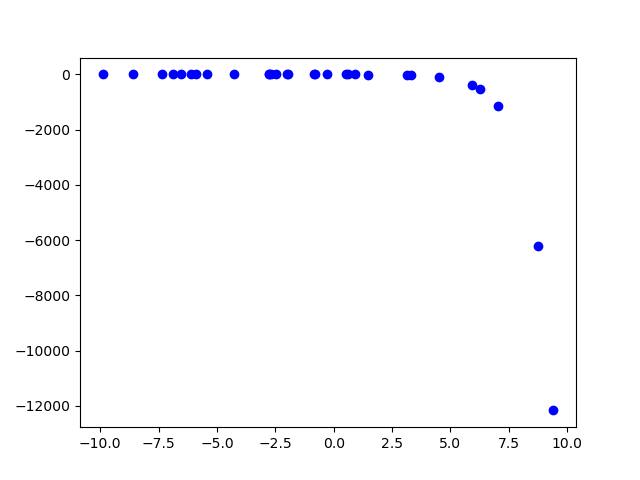
\includegraphics[width=0.5\textwidth]{../Figures/identifyModelGraph12CopyB.png}
\end{center}
\begin{enumerate}[label=\Alph*.]
\item \( \text{Exponential model} \)
\item \( \text{Non-linear Power model} \)
\item \( \text{Logarithmic model} \)
\item \( \text{Linear model} \)
\item \( \text{None of the above} \)

\end{enumerate} }
\litem{
Solve the modeling problem below, if possible.
\begin{center}
    \textit{ A new virus is spreading throughout the world. There were initially 8 many cases reported, but the number of confirmed cases has doubled every 3 days. How long will it be until there are at least 100000 confirmed cases? }
\end{center}
\begin{enumerate}[label=\Alph*.]
\item \( \text{About } 41 \text{ days} \)
\item \( \text{About } 29 \text{ days} \)
\item \( \text{About } 12 \text{ days} \)
\item \( \text{About } 13 \text{ days} \)
\item \( \text{There is not enough information to solve the problem.} \)

\end{enumerate} }
\litem{
Solve the modeling problem below, if possible.
\begin{center}
    \textit{ In CHM2045L, Brittany created a 23 liter 11 percent solution of chemical $\chi$ using two different solution percentages of chemical $\chi$. When she went to write her lab report, she realized she forgot to write the amount of each solution she used! If she remembers she used 9 percent and 22 percent solutions, what was the amount she used of the 22 percent solution? }
\end{center}
\begin{enumerate}[label=\Alph*.]
\item \( 3.54 liters \)
\item \( 11.50 liters \)
\item \( 19.46 liters \)
\item \( 7.88 liters \)
\item \( \text{There is not enough information to solve the problem.} \)

\end{enumerate} }
\litem{
For the scenario below, find the variation constant $k$ of the model (if possible).
\begin{center}
    \textit{ In an alternative galaxy, the quartic of the time, $T$ (Earth years), required for a planet to orbit Sun $\chi$ decreases as the square of the distance, $d$ (AUs), that the planet is from Sun $\chi$ decreases. For example, when Ea's average distance from Sun $\chi$ is 8, it takes 89 Earth days to complete an orbit. }
\end{center}
\begin{enumerate}[label=\Alph*.]
\item \( k = 980347.516 \)
\item \( k = 4.028 \)
\item \( k = 4015503424.000 \)
\item \( k = 1.086 \)
\item \( \text{Unable to compute the constant based on the information given.} \)

\end{enumerate} }
\litem{
Using the situation below, construct a linear model that describes the cost of the coffee beans $C(h)$ in terms of the weight of the low-quality coffee beans $h$.
\begin{center}
    \textit{ Veronica needs to prepare 120 of blended coffee beans selling for \$6.11 per pound. She has a high-quality bean that sells for \$7.57 a pound and a low-quality bean that sells for \$4.86 a pound. }
\end{center}
\begin{enumerate}[label=\Alph*.]
\item \( C(h) = 6.21 h \)
\item \( C(h) = 2.71 h + 583.20 \)
\item \( C(h) = -2.71 h + 908.40 \)
\item \( C(h) = 4.86 h \)
\item \( \text{None of the above.} \)

\end{enumerate} }
\litem{
Determine the appropriate model for the graph of points below.
\begin{center}
    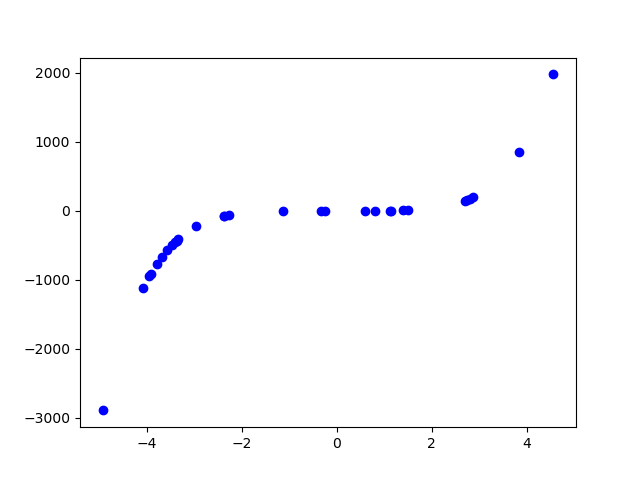
\includegraphics[width=0.5\textwidth]{../Figures/identifyModelGraph12B.png}
\end{center}
\begin{enumerate}[label=\Alph*.]
\item \( \text{Logarithmic model} \)
\item \( \text{Linear model} \)
\item \( \text{Non-linear Power model} \)
\item \( \text{Exponential model} \)
\item \( \text{None of the above} \)

\end{enumerate} }
\litem{
Solve the modeling problem below, if possible.
\begin{center}
    \textit{ A new virus is spreading throughout the world. There were initially 5 many cases reported, but the number of confirmed cases has quadrupled every 3 days. How long will it be until there are at least 10000 confirmed cases? }
\end{center}
\begin{enumerate}[label=\Alph*.]
\item \( \text{About } 23 \text{ days} \)
\item \( \text{About } 10 \text{ days} \)
\item \( \text{About } 17 \text{ days} \)
\item \( \text{About } 11 \text{ days} \)
\item \( \text{There is not enough information to solve the problem.} \)

\end{enumerate} }
\litem{
Solve the modeling problem below, if possible.
\begin{center}
    \textit{ In CHM2045L, Brittany created a 29 liter 27 percent solution of chemical $\chi$ using two different solution percentages of chemical $\chi$. When she went to write her lab report, she realized she forgot to write the amount of each solution she used! If she remembers she used 17 percent and 39 percent solutions, what was the amount she used of the 39 percent solution? }
\end{center}
\begin{enumerate}[label=\Alph*.]
\item \( 13.63 liters \)
\item \( 14.50 liters \)
\item \( 15.82 liters \)
\item \( 13.18 liters \)
\item \( \text{There is not enough information to solve the problem.} \)

\end{enumerate} }
\end{enumerate}

\end{document}